% Chapter 2
\chapter{Eclipsing Binaries and Their Period Changes} % Main chapter title
\label{ch:EB} % For referencing the chapter elsewhere, use \ref{Chapter1} 

%----------------------------------------------------------------------------------------
% Define some commands to keep the formatting separated from the content 
\newcommand{\keyword}[1]{\textbf{#1}}
\newcommand{\tabhead}[1]{\textbf{#1}}
\newcommand{\code}[1]{\texttt{#1}}
\newcommand{\file}[1]{\texttt{\bfseries#1}}
\newcommand{\option}[1]{\texttt{\itshape#1}}
%----------------------------------------------------------------------------------------

Eclipsing binaries are periodic variable stars (the cycle of variation repeats relatively reliably). 
This broad group was historically divided into three phenomenological
classes according to the appearance of the light curves: Algols, $\beta$ Lyrae systems, and W Ursae Majoris systems.
 
On the other side, morphological classification based on the Roche equipotentials provide more physical insight. Associated with the
concept of equipotentials are “limiting surfaces” or “limiting lobes.” A limiting
lobe is the volume enclosed by a limiting surface. The usefulness of morphological
classifications is that each of the stable configurations is generated by a structural-evolutionary process.

There is some correspondence between the morphological classification based on
the Roche lobes and the phenomenological classification (see section \ref{EB_classif}):
\begin{center}
Algol-type light curves $\Rightarrow$ detached and semi-detached systems\\
W UMa-type light curves $\Rightarrow$ over-contact systems.\\
\end{center}

Phenomenological classification of the $\beta$ Lyrae-type light curve has
no morphological counterpart. Sometimes, $\beta$ Lyrae-type light curves are produced
by detached systems, sometimes by semi-detached systems, and sometimes also by
systems having marginal over-contact. However, there are semi-detached binaries that are not
Algols (e.g., cataclysmic variables) and over-contact binaries that are not W UMa’s.

The characteristics of EB types according to morphological classification will be
discussed in the following section.


\section{Eclipsing Binaries Systems Classification}
\label{EB_classif}
The dynamic forces controlling the stellar mass distributions involve the effects of
rotation, tides, and non-circular orbits. For an introductory-level discussion of all
these effects, see \cite{wilson1974}. Fortunately, tidal forces produce circular orbits and
synchronous rotation in many interacting binaries. A detailed and excellent analysis
of the tidal evolution in close binary systems is provided by \cite{hut1981}. The orbital
period of a synchronous rotator in a circular orbit is the same as the rotation period.
We will discuss only synchronous rotation.

Another physical simplification reduces the mathematical complexity: although
the stars may be relatively large and considerably distorted, they attract one another
nearly as if their entire masses were concentrated into mass points at their centres. 
Therefore, only two forces need to be considered in the circular orbit and
synchronous rotation case: (i) gravitational attractions of two mass points;
(ii) the centrifugal force due to the rotation of the entire binary system about its centre of mass.
These two forces produce gravitational potential, which can be written in the form:
\begin{equation} \label{eq:roche_pot}  % Zasov "Obshchaja astrophys" p.212
\Omega_{R} = \dfrac{2}{(1+q)(r_{1}/a)}+\dfrac{2}{(1+q)(r_{2}/a)} + \dfrac{(x-\mu a)^{2}+y^{2}}{a^{2}}
\end{equation}
where\\ 
$q = M_{1}/M_{2}$,\\ 
$a=a_{1}+a_{2}$, \\
$r_{1}= \sqrt{x^{2}+y^{2}+z^{2}}$ ~and~ $r_{2}= \sqrt{(x-a)^{2}+y^{2}+z^{2}}$, \\
$\mu = M_{2}/(M_{1}+M_{2})$ \\

Given that both gravitational and centrifugal forces are time-wise constant for co-rotating 
matter, we can expect to find solutions for static configurations in the co-rotating frame. 
A somewhat similar problem was solved by the French mathematician Roche (1820--1883) in the nineteenth century. 
The basic concept for understanding the solutions of that problem is equipotential surfaces
(briefly, equipotentials). These are surfaces on which the sum of rotational and
gravitational energy per unit mass is constant. On these level surfaces, also called
\textquote{Roche surfaces}, the component of the force vector tangential to these surfaces vanishes, i.e., 
the local force vector is everywhere normal to them. The Roche surfaces
are indeed the static surfaces we are interested in: they co-rotate with the orbital
motion of the binary. Binary component surfaces are now modelled as equipotentials
(similarly on Earth, where ocean and lake surfaces follow equipotentials).

If one of the stars slowly expands, due to evolution, it will eventually fill its
Roche lobe. If the star expands further, the \textquote{path of least resistance} for the expanding matter
is through the inner Lagrangian point -- called $L_{1}$ -- into the Roche lobe of the
other star; the Roche lobe will overflow. The material falls toward the other star,
but, since it is carrying angular momentum, it falls in a spiral pattern.
There are five Lagrangian points, labelled $L_{1}$ to $L_{5}$, all in the orbital plane of the two main bodies. The first three are on the line connecting the two main bodies.
The last two, $L_{4}$ and $L_{5}$, each form an equilateral triangle with the two main bodies. The two latter points are stable, which implies that objects can orbit around them in a rotating coordinate system tied to the two main bodies \citep{Percy2007}.

The degree of star and Roche lobe contact is measured by the contact parameter, $f$ , sometimes
called the fill-out factor:
\begin{equation}
f = \dfrac{\Omega^{I}-\Omega}{\Omega^{I}-\Omega^{O}}, ~~~ \Omega^{I}\leq \Omega^{O}
\end{equation}
where $\Omega^{I}$ and $\Omega^{O}$ are modified potentials at the inner and outer Lagrangian surfaces respectively. 
%In a system of two orbiting stars, the gravitational potential energy is constant on the surfaces.
%Close to each star, the surfaces are almost spherical. But there is a \textquote{critical}
%surface -- the one which is hour-glass shaped (or figure-eight shaped, for those not familiar with hour-glasses, though, 
%as noted below, the surfaces are three-dimensional like an hour-glass, not two-dimensional like a figure eight). 
%The two halves of the hour-glass are called Roche lobes. The point of intersection
%of the hour-glasses is the inner Lagrangian point.
%https://ru.wikipedia.org/wiki/%D0%9F%D0%BE%D0%BB%D0%BE%D1%81%D1%82%D1%8C_%D0%A0%D0%BE%D1%88%D0%B0
%https://ru.wikipedia.org/wiki/%D0%A2%D0%BE%D1%87%D0%BA%D0%B8_%D0%9B%D0%B0%D0%B3%D1%80%D0%B0%D0%BD%D0%B6%D0%B0
%https://en.wikipedia.org/wiki/Lagrangian_point

According to Roche lobe fill by its star eclipsing binaries are classified to:
\begin{enumerate}
\item \textbf{detached systems} (Fig.\ref{fig:eb_det}), if neither component fills its Roche lobe.
The fill-out factor of each component is negative. If the components are small compared with their 
Roche lobes, their shapes closely approximate spheres. Whereas morphology and evolutionary state are related 
for semi-detached and over-contact binaries, such a connection does not exist in detached systems;
\item \textbf{semi-detached systems} (Fig.\ref{fig:eb_semidet}), %if one component fills its Roche lobe, and the other does not;
with one component within its critical lobe, whereas the other exactly fills its lobe ($f = 0$ for this component). This morphological
type includes Algols, cataclysmic variables, and some X-ray binaries, in which
one component is highly evolved and in which mass transfer occurs. In general, the lobe-filling star can
lose matter through the inner Lagrangian point;
\item \textbf{over-contact systems} (Fig.\ref{fig:eb_overcont}) %, if both components exceed their Roche lobes.
or common envelope binaries, where each component has
a surface larger than its Roche lobe. Mechanical equilibrium requires that the sur-
faces match in potential. That is, the common surface must coincide with a single
equipotential above the Roche lobes ($0 < f_{1,2} \leq 1$,~and~$f_{1} = f_{2}$). Configurations
are limited by the outer Lagrangian surface. This morphological type explains W UMa stars very well \citep{kallrath2009eclipsing}. %p107, 112
\end{enumerate}

\begin{figure}[!t]
\vspace{0cm}
\centerline{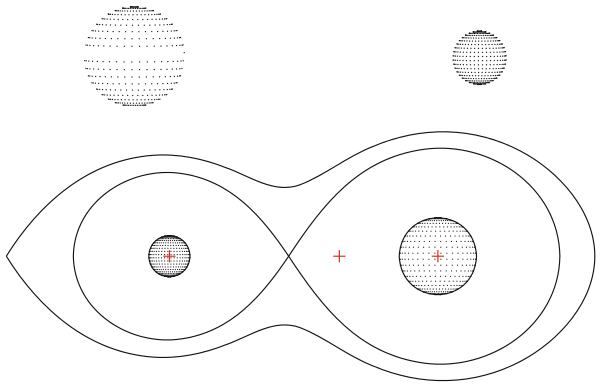
\includegraphics[width=0.56\textwidth]{EB_detached.png}}
\caption{Roche potential and shape of a detached binary system. The plot has been produced using Binary Maker 3.0 and 
the YZ Cassiopeia parameter set provided in the examples collection \citep{bradstreet2005}.($f_{1}<0, f_{2} < 0$)}
\label{fig:eb_det}
\end{figure}
\begin{figure}[!t]
\vspace{0cm}
\centerline{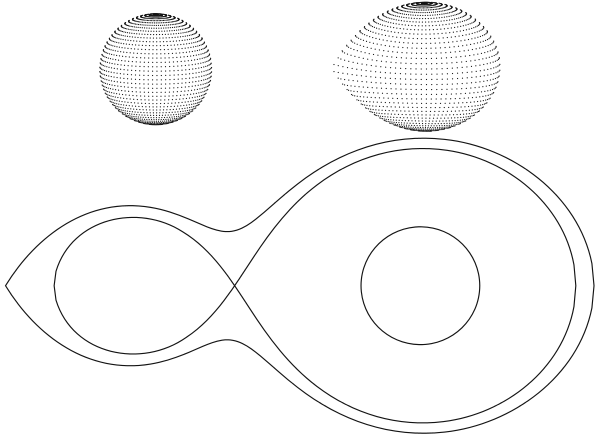
\includegraphics[width=0.56\textwidth]{EB_semidet.png}}
\caption{Roche potential and shape of a semi-detached binary. The plot has been produced with
Binary Maker 2.0 using the Algol parameter set in the examples collection \citep{bradstreet1993}. The primary component fills its Roche lobe 
($f_{1} = 0, f_{2} < 0$)}
\label{fig:eb_semidet}
\end{figure}
\begin{figure}[!t]
\vspace{0cm}
\centerline{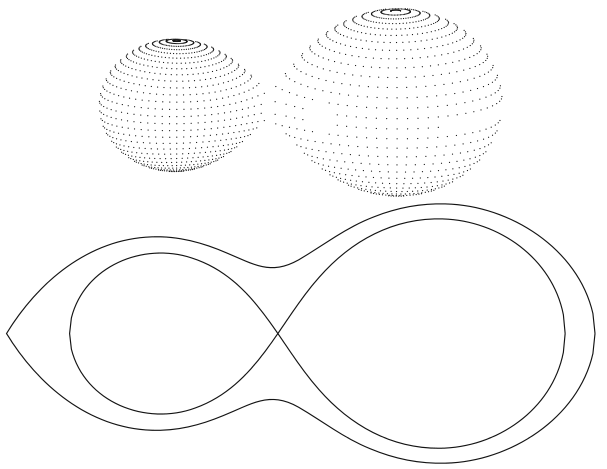
\includegraphics[width=0.56\textwidth]{EB_overcont.png}}
\caption{Roche potential and shape of an over-contact binary. The plot has been produced with
Binary Maker 2.0 for the TY Bootis parameter set in the examples collection \citep{bradstreet1993}.
Both components exceed their Roche lobes. ($0<f_{1,2}\leq1, f_{2} =f_{1}$)}
\label{fig:eb_overcont}
\end{figure}

%\section{Why Binary Stars Are Important}
\section{The Importance of Binary Stars}
Binary stars are important, first, because they are numerous. \cite{latham1992} 
conclude that the frequency of spectroscopic binaries detected in the galactic
halo is not significantly different from that in the disk, despite differences in
kinematic properties and chemical composition. The observed frequency is approximately
20\%; the actual frequency is higher because many binaries remain undetected.
In the solar neighborhood, where we have the benefit of proximity so that
proper motion variations can be detected, the frequency is more than 50\% -- and
several stars are in fact multiple systems.
The second reason why binaries are important is that they are the primary source
of our knowledge of the fundamental properties of stars. For example, the direct
determination of the mass of any astronomical object requires measurable gravitational
interaction between at least two objects (galaxy-galaxy, star-star, star-planet,
planet-satellite). In galaxy-galaxy interactions, the distances and separations are
so large that no detectable motion on the plane of the sky is possible. In star-planet
interactions, the objects contrast so greatly in brightness that outside the solar system
only the highest possible precision can resolve the objects. 
Typically in the latter case, only the star's motions are detectable, and the
properties of that star must be assumed, mainly on the basis of binary star studies, in
order to deduce the properties of the planet. In star-star interactions, the variations
in position and velocity caused by orbital motion are detectable for a wide range
of stellar separations and up to at least a factor of 5 in brightness. It is often the
case that both stars may be studied in any of several ways, depending on their distances,
brightnesses, and motions. Other basic properties of stars and of the systems
they constitute can be determined through analysis of observational data, depending
on the observational technique by which the interaction is studied \citep{kallrath2009eclipsing}. 

The full determination of absolute eclipsing binary parameters requires both a
light curve and a radial-velocity curve for each component. EBs are informative
objects because they allow photometry and spectroscopy to be combined effectively.
Eclipsing, double-lined systems are rare but very valuable. If the data quality is high
and the binary configuration is well conditioned, we have a fundamental source of
information about sizes, masses, luminosities, and distances or parallaxes of stars.
Many other parameters can be determined from precise light curve data if the configuration 
fulfills certain requirements, for example, by having complete eclipses.
Because such stars may be found over the full range of ages, they also tell how stars
evolve -- at least in binary stars \citep{kallrath2009eclipsing}.


\section{EB Systems Period Change}
\label{ch:EB_p}
Period changes in binary systems are generally due to one of three
mechanisms.
\begin{enumerate}[label=(\roman*)]
\item A loss of angular momentum from the system, or mass transfer.

\item The presence of a third body in a long orbit around the binary.
This affects the light traveltime, which can be misinterpreted as
a change in the binary period. For example, as the binary moves
towards the observer, the eclipses are seen to occur more frequently
than when the binary is moving away.

\item Applegate’s (1992) mechanism, where period changes are
caused by coupling between the binary period and changes in the
shape of the secondary star.
\end{enumerate}

% % %mass transfer
The most frequently mentioned explanation for period changes
in close binary systems is the transfer of mass from one star to another.
In \cite{Nanouris2011} authors present a equation \ref{eq:orb_angm} that reveals a close connection between the orbital angular momentum and the period of the system. Non-conservative
mass loss mechanisms increase the orbital period, while angular momentum loss processes, such as magnetic breaking and gravitational
radiation, lead to a period reduction.

\begin{equation}
\label{eq:orb_angm}
J_{orb} = \frac{M_1 M_2 G^{2/3}}{(2\pi)^{1/3}(M_1+M_2)^{1/3}}P^{1/3}
\end{equation}

From \cite{Tran2013} relation between mass transfer and amplitude of O-C modulations can be represented as:
\begin{equation}
\frac{\dot{M}}{M} \approx 4\pi^2 \frac{Amp}{T^2} 
\end{equation}
where $Amp$ and $T$ are rough measures of the amplitude and cycle time of the wave in the O-C curve.

%The most frequently mentioned explanation for period changes
%in close binary systems is the transfer of mass from one star to another. 
%However, mass transfer from a less massive to a more massive component results in a steadily increasing
%period not an alternating sequence of period increases and decreases. Mass transfer also appears to be an unsuitable
%explanation for the cyclic O-C pattern seen in close binaries for another reason. 
%The RS CVn systems, in which cyclic O-C patterns are present, are in general detached systems (Hall 1976), 
%so mass transfer cannot be invoked.
%Mass loss due to stellar winds also appears to be ruled out.
%DeCampli \& Baliunas (1979) have shown that, for RS CVn stars, the mass-loss rates required to produce a quasi-periodic signal in 
%the O-C diagram are orders of magnitude larger than allowed by observations. 
%They note that such losses would conflict with the detection of soft X-rays from
%$\alfa$ Aur, UX Ari, HR 1099, and RS CVn. 
%If we assume a single process produces the cyclic O-C curves, neither of these processes appear to be viable.
%
%
%The period change can also be explained by angular momentum loss from the binary system. Angular momentum loss is governed by two mechanisms -- gravitational radiation and magnetic braking. 
%The rates of angular momentum loss caused by both mechanisms must be added together to find the total angular momentum loss for the
%system. 
%
%The expression for gravitational radiation is given by \cite{Brinkworth2006}:
%\begin{equation}
%\left( \frac{dJ}{dt} \right)_{grav}=-\frac{32}{5} \frac{G^{7/2}}{c^5}a^{-7/2}M_1^2 M_2^2 M^{1/2}
%\end{equation}
%where $M_1$, $M_2$ and $M$ are the primary mass, secondary mass
%and total mass, respectively, and $a$ is the binary separation given
%by Newton’s form of Kepler’s third law $a = (G M/ω^2)^{1/3}$
%
%The standard model for magnetic braking in CVs is based upon
%studies of the solar wind and the rotation periods of solar-type stars
%in open clusters (Weber \& Davis 1967; Skumanich 1972; Mestel \&
%Spruit 1987). Rappaport et al. (1983) developed an empirical prescription that is still commonly used in CV studies. This relationship
%is given by
%\begin{equation}
%\left( \frac{dJ}{dt} \right)_{mb}=-3.8 \times 10^{30} M_\odot R_\odot^4 m_2 r_2^\gamma \omega^3 ~erg
%\end{equation}
%where $0\leq \gamma \leq 4$ is a dimensionless parameter and $\omega$ is the angular
%frequency of rotation of secondary star in $rad~s^{−1}$.

% % % 3 body
Apparent changes in the orbital periods of binary stars have often been attributed to the light travel time variation caused by third
bodies although further observation usually reveals that this cannot be the case.
Changes in eclipse timings of binary stars do not necessarily
indicate a genuine change in the binary period. 
A third body in a long orbit around the binary can cause small but significant changes in the
light travel time from the binary system, which manifest themselves
as strictly sinusoidal changes in the timings of mid-eclipse \cite{Brinkworth2006}.
Amplitude of light travel time variation caused by third
body than can be expressed as:
\begin{equation}
K = \frac{M_3 G^{1/3}}{c} \left[\frac{P_3}{2\pi(M_1+M_2)} \right]^{2/3}
\end{equation}
where $M_3$ is a mass of third body; $P_3$ - period of third body; $M_1, M_2$ - massses of primary and secondary components of EB system;  $G$ - gravitational constant; $c$ - speed of light (see \cite{Pribula2012} for details).

% % %Applgate
Quasi-periodic variations in eclipse times over timescales of years to decades in the orbital periods of 
eclipsing binary stars is known as the Applegate effect \cite{Applegate1992}. 
This mechanism invokes magnetic activity cycles in the low-mass components of such
binaries to redistribute angular momentum within the interior of the star, thereby changing the stellar quadrupole moment which leads to changes in the orbital period of the components. Later, \cite{Lanza1998} proposed
that the Applegate mechanism could also be driven by effectively converting rotational kinetic energy and magnetic
energy back and forth. Regardless of the details of the exact physical mechanism at work, the Applegate effect should
also operate in most exoplanet systems since the host stars are (by selection) low-mass stars with a convective outer
layer which should exhibit some form of dynamo activity \cite{Watson2010}.
%It will therefore be important to know the magnitude of the Applegate effect for exoplanet systems when interpreting any TTVs. 
According to Applegate mechanism, solar-like magnetic cycles would result in shape
changes of the low-mass components, thus redistributing the angular momentum within
the interior of the star. Then, the oblateness is changed, causing a change of the stellar
quadrupole moment which consequently leads to the variation of orbital period. 
The amplitude of orbital period modulation and the amplitude of
the oscillation in the O-C diagram are related by equation
\begin{equation}
\frac{\Delta P}{P} =2\pi \frac{A}{P_{mod}}
\end{equation}
where $A$ and $P_{mod}$ are the amplitude and modulation period of the cyclic oscillation
of the orbital period, and $\frac{\Delta P}{P}$ - period change.
% % % % % % % % % % % % % % % % % % % % % % %

%Several hypotheses have been advanced to explain the cyclic period changes in close binaries. Apsidal motion,
%which involves a change in the orientation of the binary’s major axis, is an unlikely mechanism because close binaries
%possess circular orbits, and this phenomenon only occurs in systems having large eccentricities. 
%If apsidal motion were present, the times for secondary and primary minima would be shifted in opposite directions, 
%but this effect is rarely seen and does not appear to be present in Algols. 
%An alternate possibility is that the cyclic pattern in the O-C plot is
%caused by the presence of a third body. This idea has been explored by several investigators, most recently by Borkovits \& Hegedu¨s (1996). These researchers postulate that the motion of the binary around the center of mass of a triple
%system causes the primary and secondary eclipse times to vary in a uniform and periodic fashion. In this case, the
%cyclic O-C pattern arises from orbital-induced changes in the distance to the observer. 
%Finally, Hall (1989) noted that, for Algols that possess alternating period increases and decreases, the spectral types of 
%the secondaries are always in the range late F to K. 
%These stars have outer convective zones and, if they are rapidly rotating, a magnetic dynamo
%is produced (Parker 1979). Applegate (1992) and Lanza, Rodono`, \& Rosner (1998) used this information to develop
%a theory to explain the cyclic shape of the O-C curves of these systems. They suggest that if the secondary is
%deformed by tidal and centrifugal forces, changes in the internal rotation associated with a magnetic activity cycle
%alter the star’s gravitational quadrupole moment. As the quadrupole moment increases the gravitational field
%increases, leading to a decrease in the binary period. Conversely, when the quadrupole moment decreases, the binary
%period increases (Lanza \& Rodono` 1999).